\section{Cipher Implementation}

\begin{frame}{Brief Overview}
Khazad has an SPN structure. During encryption, it iterates 8 times a SP round function. Each of this 8 rounds consists of 3 stages (except the last round):\\ 
\begin{enumerate}
        \item \textit{Nonlinear Transformation $\gamma$} 
        \item \textit{Linear Transformation $\theta$ }
        \item \textit{Adding a round key $\sigma$}
\end{enumerate}\\\\
\textbf{NOTE:-}\\
The last round does not have a linear transformation layer. 
\end{frame}

\begin{frame}{Key Expansion}
A 128-bit (16-byte) key K is divided into 2 equal parts:\\
$k_{-1}$ - older 8 bytes (from the 15th to the 8th)\\
$k_{-2}$ - lower 8 bytes (from the 7th to the 0th)\\
Keys $k_{0} \ .\ .\ . \ k_{8}$ calculated according to the Feistel scheme : \\
 $k_{i} = f(C_{i}, k_{i-1}) \oplus k_{i-2}$ \\
Here:\\
$f(x, y)$ - round function of the algorithm with the input block x and the key y.\\
$C_{i}$ - 64-bit constant, j which byte is $C_{i}^{j} = S (8i + j)$ \\
\end{frame}

\begin{frame}{Key Expansion}
\begin{center}
    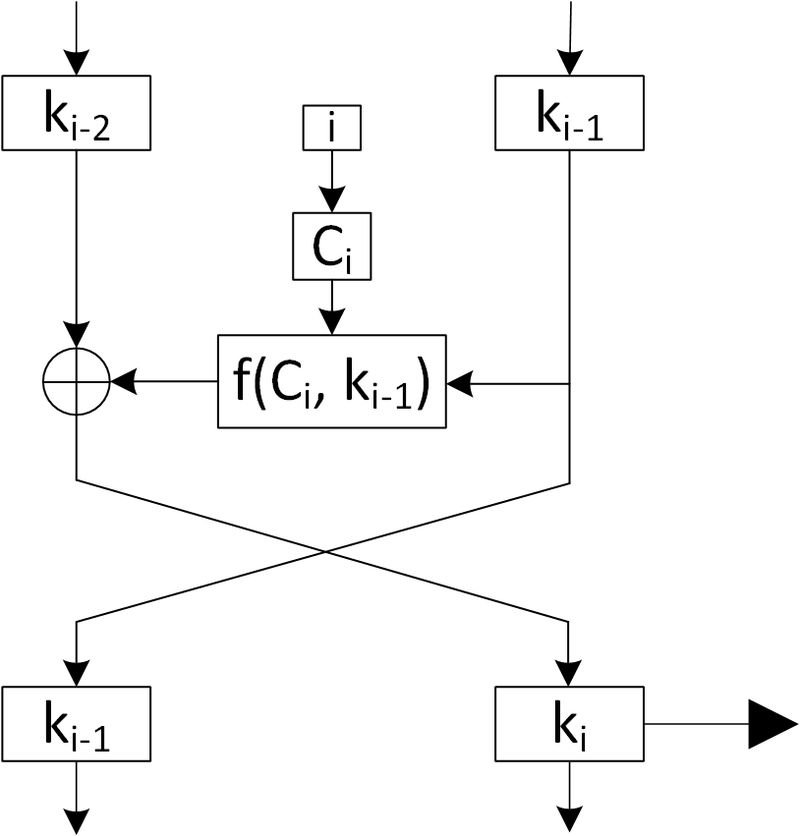
\includegraphics[scale=0.2]{Screenshots/KHAZAD_Key_Schedule_Feistel.jpg}
\end{center}
\end{frame}

\begin{frame}{Round Function}
    \begin{center}
    {\huge {Now lets see the Round function}}
    \end{center}
\end{frame}

\begin{frame}{General Round Structure}
    A single round consists of 3 stages:\\ 
    \begin{enumerate}
        \item \textit{Nonlinear Transformation ($\gamma$)} : An sbox is applied in this layer to each byte of the current state.  
        \item \textit{Linear Transformation ($\theta$ )} : The state matrix is multiplied with a square matrix in GF ($2^8$ ) of size 8
        \item \textit{Adding a round key ($\sigma$)} : The xor of the round key and the state matrix is taken in this stage.
    \end{enumerate}
\end{frame}

\begin{frame}{Nonlinear transformation ($\gamma$)}
    Denoted as $\gamma$.\\
    In each round, the input block is divided into smaller blocks of 8 bytes, which are independently subjected to nonlinear transformation (change), i.e. passed in parallel through the same S-blocks (each S-block - 8x8 bits, i.e. 8 bits at the input and 8 bits at the output).\\ 
    Replacement blocks in the source and modified (tweaked) ciphers are different. The substitution unit is selected so that the nonlinear transformation is involutionary, i.e. $\gamma = \gamma^{-1} \ or \ \gamma(\gamma(x)) = x.$
\end{frame}

\begin{frame}{Linear transformation $\theta$}
     Denoted by $\theta$. An 8-byte row of data is multiplied byte by byte to a fixed matrix H size 8 x 8, and byte multiplication is performed in the Galois field $GF(2^{8})$ with a polynomial that is not given $x^{8} + x^{4} + x^{3} + x^{2} +1 \ (0x11D)$.\\
    \begin{center}
        $\theta (x) = x \times H$ \ where\\ 
        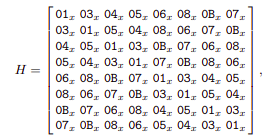
\includegraphics[scale=0.5]{Screenshots/hbox.png}
    \end{center}
    
\end{frame}

\begin{frame}{Adding a round key $\sigma$}
    A 64-bit XOR operation is performed on the 64-bit data block \& the 64-bit round key .
    A 64-bit data block is being xored with a round key of 64 bits calculated using key expansion algorithm based on Fiestal scheme.\\
   \begin{center}
       For $i^{th} \ round \ : \ \sigma (x_i) = x_{i-1} \oplus k_{i-1}$
   \end{center} 
\end{frame}

\begin{frame}{Encryption Algorithm}
    \begin{center}
        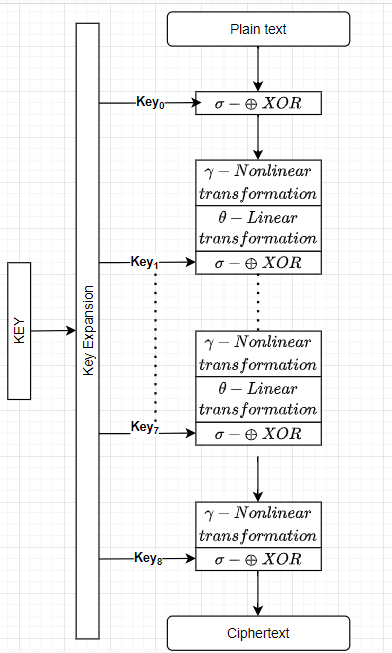
\includegraphics[scale=0.42]{Screenshots/encrypt.png}\\ 
        \textbf{The Encryption Algorithm}
    \end{center}
\end{frame}


\begin{frame}{Decryption Algorithm}
    \begin{center}
        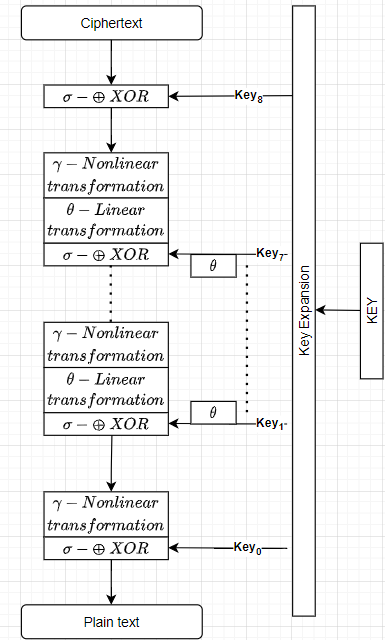
\includegraphics[scale=0.42]{Screenshots/decrypt.png} \\ 
            \textbf{The Decryption Algorithm}
    \end{center}
\end{frame}
